
Two different approaches can be found to improve Java bytecode
execution by hardware. The first type operates as a Java coprocessor
in conjunction with a general-purpose microprocessor. This
coprocessor is placed in the instruction fetch path of the main
processor and translates Java bytecodes to sequences of instructions
for the host CPU or directly executes basic Java bytecodes. The
complex instructions are emulated by the main processor. Java chips
in the second category replace the general-purpose CPU. All
applications therefore have to be written in Java. While the first
type enables systems with mixed code capabilities, the additional
component significantly raises costs.
\tablename~\ref{tab_related_proc} provides an overview of the
described Java hardware.

Blank fields in the table indicate that the information is not
available or not applicable (e.g. for simulation-only projects).
Minimum CPI is the number of clock cycles for a simple instruction
such as \code{nop}. One entry, the TINI system, is not a real Java
hardware, but is included in the table since it is often
incorrectly\footnote{TINI is a standard interpreting JVM running on
an enhanced 8051 processor.} cited as an embedded Java processor.


%\begin{table}
%    \centering
%{\footnotesize
%\begin{tabular}
%    {|>{\bfseries}p{1.4cm}|m{1.3cm}|>{\raggedright}m{1.3cm}|>{\raggedright}m{1.3cm}
%    |r|>{\raggedright}m{1.35cm}|r|m{1.6cm}|}
%
%    \hline
%         & Type & Target  & Size & Speed & Java     & Min. & Remarks \\
%         &      & technology &      & [MHz] & standard & CPI  &         \\
%    \hline
%    Hard-Int & Translation & Simulation only &  &  &  &  &  \\
%    \hline
%    DELFT & Translation & Simulation only &  &  &  &  &  \\
%    \hline
%    JIFFY & Translation & Xilinx FPGA & 3800 LCs, 1KB RAM &  &  &  &  \\
%    \hline
%    Jazelle & Co-processor & ASIC 0.18$\mu$ & 12K gates & 200 &  &  & Integration with ARM \\
%    \hline
%    JSTAR & Co-processor & ASIC 0.18$\mu$ Softcore & 30K gates + 7KB & 104 & J2ME CLDC\footnotemark[2] &  &  \\
%    \hline
%    TINI & Software JVM & Enhanced 8051 clone &  &  & Java 1.1 subset &  & A small Java system for embedded applications. \\
%    \hline
%    picoJava & Processor & No realization & 128K gates + memory &  & Full & 1 &  \\
%    \hline
%    aJile & Processor & ASIC 0.25$\mu$ & 25K gates + ROM & 100 & J2ME CLDC\footnotemark[2] &  &  \\
%    \hline
%    Cjip & Processor & ASIC 0.35$\mu$ & 70K gates + ROM, RAM & 67 & J2ME CLDC\footnotemark[2] & 6 & Rewriteable microcode \\
%    \hline
%    Ignite & Stack processor & Xilinx FPGA & 9700 LCs &  &  &  &  \\
%    \hline
%    Moon & Processor & Altera FPGA & 3660 LCs, 4KB RAM &  &  &  &  \\
%    \hline
%    Lightfoot & Processor & Xilinx FPGA & 3400 LCs & 40 &  &  &  \\
%    \hline
%    LavaCORE & Processor & Xilinx FPGA & 3800 LCs 30K gates & 20 &  &  &  \\
%    \hline
%    Komodo & Processor & Xilinx FPGA & 2600 LCs & 20 & Subset: 50 bytecodes & 4 &  \\
%    \hline
%    FemtoJava & Processor & Altera Flex 10K & 2000 LCs & 4 & Subset: 69 bytecodes, 16-bit ALU & 3 & Application specific Java processor. \\
%    \hline
%    JSM & Processor & Xilinx FPGA &  & 3.5 & Java Card &  & \cite{JSM01} \\
%    \hline
%%    \hline
%%    JOP & Processor & Altera, Xilinx FPGA & 2100 LCs + 3KB RAM & 100 & J2ME CLDC & 1 & Typical configuration on a Cyclone FPGA \\
%
%\end{tabular}
%}
%    \caption{Java hardware}
%    \label{tab_related_proc}
%\end{table}


\begin{table}
    \centering
{\footnotesize
\begin{tabular}
    {|>{\bfseries}p{1.6cm}|m{1.5cm}|>{\raggedright}m{1.6cm}|>{\raggedright}m{1.6cm}
    |r|>{\raggedright}m{1.5cm}|r|}

    \hline
         & Type & Target  & Size & Speed & Java     & Min. \\
         &      & technology &      & [MHz] & standard & CPI  \\
    \hline
    Hard-Int & Translation & Simulation only &  &  &  &  \\
    \hline
    DELFT & Translation & Simulation only &  &  &  &    \\
    \hline
    JIFFY & Translation & Xilinx FPGA & 3800 LCs, 1KB RAM &  &  &   \\
    \hline
    Jazelle & Co-processor & ASIC 0.18$\mu$ & 12K gates & 200 &  &  \\
    \hline
    JSTAR & Co-processor & ASIC 0.18$\mu$ Softcore & 30K gates + 7KB & 104 & J2ME CLDC\footnotemark[2] &  \\
    \hline
    TINI & Software JVM & Enhanced 8051 clone &  &  & Java 1.1 subset &   \\
    \hline
    picoJava & Processor & No realization & 128K gates + memory &  & Full & 1  \\
    \hline
    aJile & Processor & ASIC 0.25$\mu$ & 25K gates + ROM & 100 & J2ME CLDC\footnotemark[2] &   \\
    \hline
    Cjip & Processor & ASIC 0.35$\mu$ & 70K gates + ROM, RAM & 67 & J2ME CLDC\footnotemark[2] & 6 \\
    \hline
    Ignite & Stack processor & Xilinx FPGA & 9700 LCs &  &  &   \\
    \hline
    Moon & Processor & Altera FPGA & 3660 LCs, 4KB RAM &  &  &   \\
    \hline
    Lightfoot & Processor & Xilinx FPGA & 3400 LCs & 40 &  &   \\
    \hline
    LavaCORE & Processor & Xilinx FPGA & 3800 LCs 30K gates & 20 &  &   \\
    \hline
    Komodo & Processor & Xilinx FPGA & 2600 LCs & 20 & Subset: 50 bytecodes & 4  \\
    \hline
    FemtoJava & Processor & Altera Flex 10K & 2000 LCs & 4 & Subset: 69 bytecodes, 16-bit ALU & 3 \\
    \hline
    JSM \cite{JSM01} & Processor & Xilinx FPGA &  & 3.5 & Java Card &   \\
    \hline
%    \hline
%    JOP & Processor & Altera, Xilinx FPGA & 2100 LCs + 3KB RAM & 100 & J2ME CLDC & 1 & Typical configuration on a Cyclone FPGA \\

\end{tabular}
}
    \caption{Java hardware}
    \label{tab_related_proc}
\end{table}

\footnotetext[2]{J2ME CLDC stands for Java2 Micro Edition, Connected
Limited Device Configuration, which is described in
Section~\ref{subsec:cldc}.}


% Change this: \emph{JOP is included with a typical configuration as a
% reference. Further details of the resource usage of JOP is described
% in Section~xxx.}


\section{Hardware Translation and Coprocessors}

The simplest enhancement for Java is a translation unit, which
substitutes the switch statement of an interpreter JVM (bytecode
decoding) through hardware and/or translates simple bytecodes
to a sequence of RISC instructions on the fly.

A standard JVM interpreter contains a loop with a large switch
statement that decodes the bytecode (see
Listing~\ref{lst:intro:java:intprt}). This switch statement is
compiled to an indirect branch. The destinations of these indirect
branches change frequently and do not benefit from branch-prediction
logic. This is the main overhead for simple bytecodes on modern
processors. The following approaches enhance the execution of Java
programs on a standard processor through the substitution of the
memory read and switch statement with bytecode fetch and decode
through hardware.


\subsection{Hard-Int}

Radhakrichnan \cite{HardInt} proposes an additional architecture for
a standard RISC processor to speed up a JVM interpreter. The
architecture, called Hard-Int, is placed between the cache and
instruction fetch of the RISC processor. Simple Java bytecodes are
translated to a sequence of RISC instructions. For native RISC code,
the unit is bypassed. This architecture implements the expensive
switch statement of a typical interpreter in hardware. A simulation
of a SPARC processor with four execution units shows a speedup by
the factor of 2.6 over JDK 1.2 JIT with SPECjvm98. Since the
architecture is only evaluated in a software simulation, the impact
of the inserted hardware on the clock frequency of the RISC
processor is unknown. No estimation of the additional hardware cost
for the translation unit is given.


\subsection{DELFT-JAVA Engine}

In his thesis \cite{DELFT}, Glossner describes a processor for
multimedia applications in Java. A RISC processor is extended with
DSP capabilities and Java specific instructions. This combination
results in a very complex processor. Simple JVM instructions are
dynamically translated to the DELFT instruction set. However, no
explanation is given as to how this is done. A new
register-addressing mode, indirect register addressing with auto
increment or decrement, provides support for stack caching in the
register file. The translation of JVM bytecode to the DELFT
instruction set maps stack-based dependencies into pipeline
dependencies. The author expects that these dependencies can be
resolved with standard techniques such as register renaming and
out-of-order execution. To accelerate dynamic linking a link
translation buffer cache resolved entries from the constant pool.


The processor is validated through a C++ model. An experiment with a
synthetic benchmark (vector multiplication) compared a stack machine
with an ideal register machine. The ideal register machine performs
register renaming and out-of-order execution on multiple execution
units. The achieved speedup in this experiment was 2.7. The
high-level simulation model is more a proof of concept and no
estimation is given for the resources needed to implement this
complex processor. Since only a restricted subset of the JVM was
simulated, no Java applications could be used to estimate the
expected speedup.


\subsection{JIFFY}

An interesting approach to enhance Java execution in embedded
systems is presented in Acher's thesis \cite{JIFFY}. He states that
JIT-compilation in software is not possible on most embedded devices
because of resource constraints. JIFFY, a JIT in an FPGA, is
proposed as a solution to this problem. The compilation is done in
the following steps:

The Java bytecode is translated into an intermediate language with
three registers and a stack. The reduction to three registers is due
to the fact that bytecodes are using a maximum of three stack
operands, and it simplifies translation to CISC-architectures with a
low register count. In the next step, this instruction sequence,
which is still stack-based, is optimized. The main effect of this
optimization is to transform stack-based operations into
register-based operations. These optimized instructions in the
intermediate language are translated to native instructions of the
target architecture in the last step.

The quality of the generated code was tested with software versions
of JIFFY for a CISC (80586) and a RISC (Alpha 21164) architecture.
The resulting code is about 1.1 to 7.5 times faster than
interpreting Java bytecode on the x86 architecture. The speedup is
similar to Suns first JIT compiler (sunwjit in JDK 1.1). The
compilation time is estimated to be 50 to 70 clock cycles for one
bytecode. This is 10 times faster than the efficient CACAO JIT
\cite{Krall98}. A first prototype implementation in an FPGA used
3800 LCs and 8KBits RAM (80 \% of a Xilinx XC2S200).


\subsection{Jazelle}

Jazelle \cite{Jazelle} is an extension of the ARM 32-bit RISC
processor, similar to the Thumb state (a 16-bit mode for reduced
memory consumption). The Jazelle coprocessor is integrated into the
same chip as the ARM processor. The hardware bytecode decoder logic
is implemented in less than 12K gates. It accelerates, according to
ARM, some 95\% of the executed bytecodes. 140 bytecodes are executed
directly in hardware, while the remaining 94 are emulated by
sequences of ARM instructions. This solution also uses code
modification with \textit{quick} instructions to substitute certain
object-related instructions after link resolution. All Java
bytecodes, including the emulated sequences, are re-startable to
enable a fast interrupt response time.


A new ARM instruction puts the processor into Java state. Bytecodes
are fetched and decoded in two stages, compared to a single stage in
ARM state. Four registers of the ARM core are used to cache the top
stack elements. Stack spill and fill is handled automatically by the
hardware. Additional registers are reused for the Java stack
pointer, the variable pointer, the constant pool pointer and locale
variable 0 (the \textit{this} pointer in methods). Keeping the
complete state of the Java mode in ARM registers simplifies its
integration into existing operating systems.

\subsection{JSTAR, JA108}

Nozomi's JA108 \cite{JSTAR}, previously known as JSTAR, Java
coprocessor sits between the native processor and the memory
subsystem. JA108 fetches Java bytecodes from memory and translates
them into native microprocessor instructions. JA108 acts as a
pass-through when the core processor's native instructions are being
executed. The JA108 is targeted for use in mobile phones to increase
performance of Java multimedia applications. The coprocessor is
available as standalone package or with included memory and can be
operated up to 104MHz. The resource usage for the JSTAR is known to
be about 30K gates plus 45Kbits for the microcode.

\subsection{A Co-Designed Virtual Machine}

In his thesis \cite{KentPhD}, Kent proposes an interesting new form
of Java coprocessor. He investigates hardware/software co-design for
a JVM within the context of a desktop workstation. The execution of
the JVM is partitioned between an FPGA and the host processor. An
FPGA board with local memory is connected via the PCI bus to the
host. This solution provides an add-on accelerator without changing
the system. Moreover, as the FPGA can be configured for a different
task, the add-on hardware can be used for non-Java applications.

The critical issue in this approach is the partitioning of the JVM
and the memory regions between hardware and software. Not all Java
bytecodes can be executed in hardware. All object-oriented bytecodes
are performed in software. However, once these bytecodes are
replaced by their \textit{quick} variants, some of them can then be
executed in hardware. The most accessed data structures, i.e.\ the
method's bytecode, execution stack and local variables, are placed
in the FPGA board memory. The constant pool and the heap reside in
the PC's main memory. The software part of the JVM decides during
runtime which instruction sequences can be executed by the hardware.
Due to the high cost of a context switch, this is a critical
decision. Kent explored various algorithms with different block
sizes to find the optimum partitioning of the instructions between
the host processor and the FPGA. Tests with small benchmarks on a
simulation showed performance gains by a factor of 6 to 11, when
compared with an interpreting JVM. Kent is now working on the
concurrent use of the FPGA and the host system to execute Java
applications. Additional performance increases are expected for
multi-threaded applications.

In our view, there are two potential problems with this approach.
Firstly, the execution context for the hardware is too small. As
\code{invokevirtual} and the quick version are implemented in the
software partition, the maximum context is one method body. As shown
in Section~\ref{sec:bench:jvm:methods}, Java methods are usually
small (about 30\% are less than 9 bytes long), resulting in many
context switches. The second issue is the raw speedup, without
communication overhead, of the FPGA solution. This speedup is stated
to be around of 10 times greater, with the same clock frequency.
However, FPGA clock rate will never reach the clock rate of a
general-purpose processor. With a meaningful design, such as a CPU,
the clock rate of an FPGA is about 20 to 50 times lower. However,
everyone who uses an FPGA as target technology for a processor
design faces this problem. It is better not to try to compete
against mainstream PC technology.

\section{Java Processors}

Java Processors are primarily used in an embedded system. In such a
system, Java is the native programming language and all operating
system related code, such as device drivers, are implemented in
Java. Java processors are simple or extended stack architectures
with an instruction set that resembles more or less the bytecodes
from the JVM.

\subsection{picoJava}
\label{subsec:related:picojava}

Sun's picoJava is the Java processor most often cited in research
papers. It is used as a reference for new Java processors and as the
basis for research into improving various aspects of a Java
processor. Ironically, this processor was never released as a
product by Sun. After Sun decided to not produce picoJava in
silicon, Sun licensed picoJava to Fujitsu, IBM, LG Semicon and NEC.
However, these companies also did not produce a chip and Sun finally
provided the full Verilog code under an open-source license.

Sun introduced the first version of picoJava \cite{624084} in 1997.
The processor was targeted at the embedded systems market as a pure
Java processor with restricted support of C. picoJava-I contains
four pipeline stages. A redesign followed in 1999, known as
picoJava-II. This is the version described below. picoJava-II is now
freely available with a rich set of documentation \cite{pjMicroArch,
pjProgRef}.

Simple Java bytecodes are directly implemented in hardware, most of
them execute in one to three cycles. Other performance critical
instructions, for instance invoking a method, are implemented in
microcode. picoJava traps on the remaining complex instructions,
such as creation of an object, and emulates this instruction. To
access memory, internal registers and for cache management picoJava
implements 115 extended instructions with 2-byte opcodes. These
instructions are necessary to write system-level code to support the
JVM.

Traps are generated on interrupts, exceptions and for instruction
emulation. A trap is rather expensive and has a minimum overhead of
16 clock cycles:

\begin{verbatim}
    6 clocks trap execution
    n clocks trap code
    2 clocks set VARS register
    8 clocks return from trap
\end{verbatim}


This minimum value can only be achieved if the trap table entry is
in the data cache and the first instruction of the trap routine is
in the instruction cache. The worst-case interrupt latency is 926
clock cycles \cite{pjProgRef}.

\begin{figure*}
    \centering
%    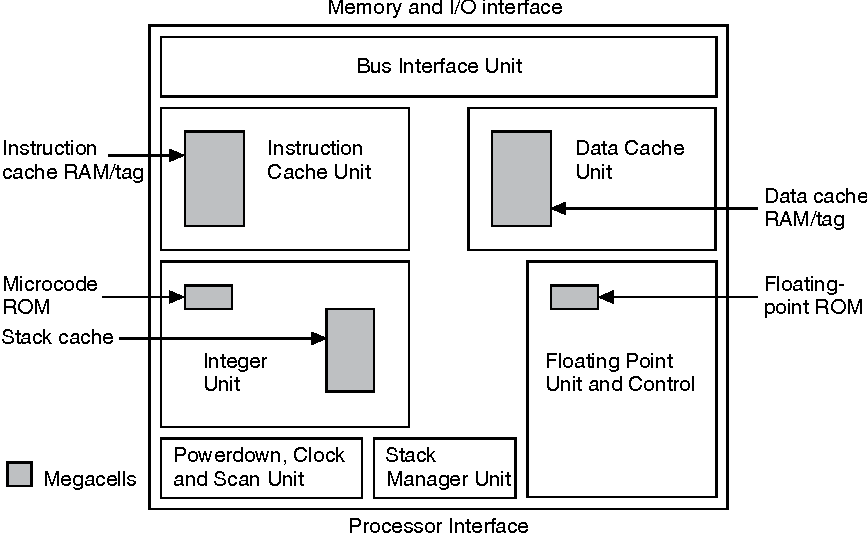
\includegraphics[scale=\picscale]{related/related_picojava}
    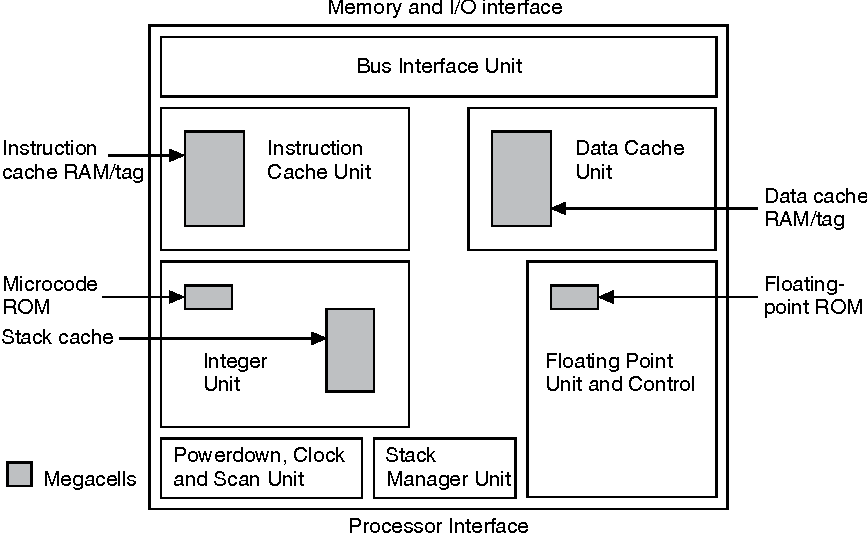
\includegraphics[scale=0.85]{related/related_picojava}
    \caption[Block diagram of picoJava-II]
    {Block diagram of picoJava-II (from \cite{pjMicroArch})}
    \label{fig_related_picojava}
\end{figure*}

\figurename~\ref{fig_related_picojava} shows the major function
units of picoJava. The integer unit decodes and executes picoJava
instructions. The instruction cache is direct-mapped, while the data
cache is two-way set-associative, both with a line size of 16 bytes.
The caches can be configured between 0 and 16 Kbytes. An instruction
buffer decouples the instruction cache from the decode unit. The FPU
is organized as a microcode engine with a 32-bit datapath supporting
single- and double-precision operations. Most single-precision
operations require four cycles. Double-precision operations require
four times the number of cycles as single-precision operations. For
low-cost designs, the FPU can be removed and the core traps on
floating-point instructions to a software routine to emulate these
instructions. picoJava provides a 64-entry stack cache as a register
file. The core manages this register file as a circular buffer, with
a pointer to the top of stack. The stack management unit
automatically performs spill to and fill from the data cache to
avoid overflow and underflow of the stack buffer. To provide this
functionality the register file contains five memory ports.
Computation needs two read ports and one write port, the concurrent
spill and fill operations the two additional read and write ports.
The processor core consists of following six pipeline stages:
%
\begin{description}

\item[Fetch:]
Fetch 8 bytes from the instruction cache or 4 bytes from the bus
interface to the 16-byte-deep prefetch buffer.

\item[Decode:]
Group and precode instructions (up to 7 bytes) from the prefetch
buffer. Instruction folding is performed on up to four bytecodes.

\item[Register:]
Read up to two operands from the register file (stack cache).

\item[Execute:]
Execute simple instructions in one cycle or microcode for
multi-cycle instructions.

\item[Cache:]
Access the data cache.

\item[Writeback:]
Write the result back into the register file.

\end{description}
%
The integer unit together with the stack unit provides a mechanism,
called instruction folding, to speed up common code patterns found
in stack architectures, as shown in
\figurename~\ref{fig_related_folding}.
%
\begin{figure}
A Java instruction
    \begin{verbatim}
    c = a + b;
    \end{verbatim}
translates to the following bytecodes:
    \begin{verbatim}
    iload_1
    iload_2
    iadd
    istore_3
    \end{verbatim}
    \caption{A common folding pattern that is executed in a single cycle}
    \label{fig_related_folding}
\end{figure}
%
When all entries are contained in the stack cache, the picoJava core
can fold these four instructions to one RISC-style single cycle
operation.

picoJava contains a simple mechanism to speed-up the common case for
monitor enter and exit. The two low order bits of an object
reference are used to indicate the lock holding or a request to a
lock held by another thread. These bits are examined by
\code{monitorenter} and \code{monitorexit}. For all other operations
on the reference, these two bits are masked out by the hardware.
Hardware registers cache up to two locks held by a single thread.

To efficiently implement a generational or an incremental garbage
collector picoJava offers hardware support for write barriers
through memory segments. The hardware checks all stores of an object
reference if this reference points to a different segment (compared
to the store address). In this case, a trap is generated and the
garbage collector can take the appropriate action. Additional two
reserved bits in the object reference can be used for a write
barrier trap.

The architecture of picoJava is a stack-based CISC processor
implementing 341 different instructions \cite{pJ1} and is the most
complex Java processor available. The processor can be implemented
\cite{Sekar2000} in about 440K gates (128K for the logic and 314K
for the memory components: 284x80 bits microcode ROM, 2x192x64 bits
FPU ROM and 2x16~KB caches). We have implemented picoJava-II in a
Cyclone-II FPGA \cite{pjfpga} and the design consumed 27500~LCs and
48~KB on-chip memory.

\subsection{aJile JEMCore}

aJile's JEMCore is a direct-execution Java processor that is
available as both an IP core and a stand alone processor
\cite{aJile, 880720}. It is based on the 32-bit JEM2 Java chip
developed by Rockwell-Collins. JEM2 is an enhanced version of JEM1,
created in 1997 by the Rockwell-Collins Advanced Architecture
Microprocessor group. Rockwell-Collins originally developed JEM for
avionics applications by adapting an existing design for a
stack-based embedded processor. Rockwell-Collins decided not to sell
the chip on the open market. Instead, it licensed the design
exclusively to aJile Systems Inc., which was founded in 1999 by
engineers from Rockwell-Collins, Centaur Technologies, Sun
Microsystems, and IDT.


The core contains 24 32-bit wide registers. Six of them are used to
cache the top elements of the stack. The datapath consists of a
32-bit ALU, a 32-bit barrel shifter and the support for floating
point operations (disassembly/assembly, overflow and NaN detection).
The control store is a 4K by 56 ROM to hold the microcode that
implements the Java bytecode. An additional RAM control store can be
used for custom instructions. This feature is used to implement the
basic synchronization and thread scheduling routines in microcode.
This results in low execution overheads with thread-to-thread yield
of less than one $\mu$s (at 100MHz). An optional Multiple JVM
Manager (MJM) supports two independent, memory protected JVMs. The
two JVMs execute time-sliced on the processor. According to aJile,
the processor can be implemented in 25K gates (without the microcode
ROM). The MJM needs additional 10K gates.

Two silicon versions of JEM exist today: the aJ-80 and the aJ-100.
Both versions comprise a JEM2 core, the MJM, 48KB zero wait state
RAM and peripheral components, such as timer and UART. 16KB of the
RAM is used for the writable control store. The remaining 32KB is
used for storage of the processor stack. The aJ-100 provides a
generic 8-bit, 16-bit or 32-bit external bus interface, while the
aJ-80 only provides an 8-bit interface. The aJ-100 can be clocked up
to 100MHz and the aJ-80 up to 66MHz. The power consumption is about
1mW per MHz.

Since aJile was a member of the Real-Time for Java Expert Group, the
complete RTSJ will be available in the near future. One nice feature
of this processor is its availability. A relatively cheap
development system, the JStamp \cite{JStamp}, was used to compare
this processor with JOP.

\subsection{Cjip}

The Cjip processor \cite{Imsys, Cjip} supports multiple instruction
sets, allowing Java, C, C++ and assembler to coexist. Internally,
the Cjip uses 72 bit wide microcode instructions, to support the
different instruction sets. At its core, Cjip is a 16-bit CISC
architecture with on-chip 36KB ROM and 18KB RAM for fixed and
loadable microcode. Another 1KB RAM is used for eight independent
register banks, string buffer and two stack caches. Cjip is
implemented in 0.35-micron technology and can be clocked up to
66MHz. The logic core consumes about 20\% of the
1.4-million-transistor chip. The Cjip has 40 program controlled I/O
pins, a high-speed 8 bit I/O bus with hardware DMA and an 8/16 bit
DRAM interface.


The JVM is implemented largely in microcode (about 88\% of the Java
bytecodes). Java thread scheduling and garbage collection are
implemented as processes in microcode. Microcode is also used to
implement virtual peripherals such as watchdog timers, display and
keyboard interfaces, sound generators and multimedia codecs.

Microcode instructions execute in two or three cycles. A JVM
bytecode requires several microcode instructions. The Cjip Java
instruction set and the extensions are described in detail in
\cite{CjipRef}. For example: a bytecode \code{nop} executes in 6
cycles while an \code{iadd} takes 12 cycles. Conditional bytecode
branches are executed in 33 to 36 cycles. Object oriented
instructions such \code{getfield}, \code{putfield} or
\code{invokevirtual} are not part of the instruction set.


\subsection{Ignite, PSC1000}

The PSC1000 \cite{IGNITE} is a stack processor, based on ShBoom
(originally designed by Chuck Moore \cite{ShBoom}), designed for
high speed Forth applications. The PSC1000 was later renamed to
Ignite and promoted as a Java-processor, though it has it roots in
Forth. The instruction set, called ROSC (Removed Operand Set
Computer), is different from Java bytecodes. A small JVM driver
converts Java bytecode into the stack instruction set of the
processor.


The processor contains two on-chip stacks, as usual in Forth
processors \cite{Koopman89}, and additional 16 global registers. The
first elements of the stacks are directly accessible. The bottleneck
of instruction fetching without a cache is avoided by fetching up to
four 8-bit instructions from a 32-bit memory. To simplify
instruction decoding immediate values and branch offsets are placed
right aligned in such an instruction group. The PSC1000 is available
as ASIC at 80MHz and as a soft-core for Xilinx FPGAs (9700 LCs).


\subsection{Moon}

Vulcan ASIC's Moon processor is an implementation of the JVM to run
in an FPGA. The execution model is the often-used mix of direct,
microcode and trapped execution. As described in \cite{Vulcan2000},
a simple stack folding is implemented in order to reduce five memory
cycles to three for instruction sequences like
\textit{push-push-add}. The first version of Moon uses 3.840 LCs and
10 embedded memory blocks in an Altera FPGA. The Moon2 processor
\cite{Vulcan2003} is available as an encrypted HDL source for Altera
FPGAs (22\% of an APEX 20K400E equates to 3660 LCs) or as VHDL or
Verilog source code. The minimum silicon cost is given as 27K gates
plus 3KB ROM and 1KB single port RAM. The single port RAM is used to
implement 256 entries of the stack.


\subsection{Lightfoot}

The Lightfoot 32-bit core \cite{Lightfoot} is a hybrid 8/32-bit
processor based on the Harvard architecture. Program memory is 8
bits wide and data memory is 32 bits wide. The core contains a
3-stage pipeline with an integer ALU, a barrel shifter and a 2-bit
multiply step unit. There are two different stacks with top elements
implemented as registers and memory extension. The data stack is
used to hold temporary data -- it is not used to implement the JVM
stack frame. As the name implies, the return stack holds return
addresses for subroutines and it can be used as an auxiliary stack.
The TOS element is also used to access memory. The processor
architecture specifies three different instruction formats: soft
bytecodes, non-returnable instructions and single-byte instructions
that can be folded with a return instruction. Soft bytecode
instructions cause the processor to branch to one of 128 locations
in low program memory, where the implementation of the soft
bytecodes resides. This operation has a single cycle overhead and
the address of the following instruction is pushed onto the return
stack. The instruction set implies that it is optimized to write an
efficient interpreted JVM.


The core is available in VHDL and can be implemented in less than
30K gates. According to DCT, the performance is typically 8 times
better than RISC interpreters running at the same clock speed. The
core is also provided as an EDIF netlist for dedicated Xilinx
devices. It needs 1710 CLBs (= 3400 LCs) and 2 Block RAMs. In a
Vertex-II (2V1000-5), it can be clocked up to 40MHz.


\subsection{LavaCORE}

LavaCORE \cite{LavaCORE} is another Java processor targeted at
Xilinx FPGA architectures. It implements a set of instructions in
hardware and firmware. Floating-point operations are not
implemented. A 32x32-bit dual-ported RAM implements a register-file.
For specialized embedded applications, a tool is provided to analyze
which subset of the JVM instructions is used. The unused
instructions can be omitted from the design. The core can be
implemented in 1926 CLBs (= 3800 LCs) in a Virtex-II (2V1000-5) and
runs at 20MHz.

\subsection{Komodo}
\label{subsec:related:komodo}

Komodo \cite{Zulauf00} is a multithreaded Java processor with a
four-stage pipeline. It is intended as a basis for research on
real-time scheduling on a multithreaded microcontroller
\cite{komodo2003}. Simple bytecodes are directly implemented, while
more complex bytecodes, such as \code{iaload}, are implemented as a
microcode sequence. The unique feature of Komodo is the instruction
fetch unit with four independent program counters and status flags
for four threads. A priority manager is responsible for hardware
real-time scheduling and can select a new thread after each bytecode
instruction.


The first version of Komodo in an FPGA implements a very restricted
subset of the JVM (only 50 bytecodes). The design can be clocked at
20MHz. However, the pipeline runs at 5MHz for single cycle external
memory access and three-port access of stack memory in one pipeline
stage. The resource usage is 1300 CLBs (= 2600 LCs) in a Xilinix XC
4036 XL.

\subsection{FemtoJava}

FemtoJava \cite{Femto01} is a research project to build an
application specific Java processor. The bytecode usage of the
embedded application is analyzed and a customized version of
FemtoJava is generated. FemtoJava implements up to 69 bytecode
instructions for an 8 or 16 bit datapath. These instructions take 3,
4, 7 or 14 cycles to execute. Analysis of small applications (50 to
280 byte code) showed that between 22 and 69 distinct bytecodes are
used. The resulting resource usage of the FPGA varies between 1000
and 2000 LCs. With the reduction of the datapath to 16 bits the
processor is not Java conformant.

\subsection{jHISC}

The jHISC project \cite{jHISC:jnl2006} proposes a high-level
instruction set architecture for Java. This project is closely
related to picoJava. The processor consumes 15500~LCs in an FPGA and
the maximum frequency in a Xilinx Virtex FPGA is 30~MHz.
%
%However, the resulting design is probably not very well balanced.
%The processor consumes 15500 LCs compared to about 3000 LCs for JOP.
%The maximum frequency in a Xilinx Virtex FPGA is 30 MHz compared to
%100 MHz for JOP.
%
According to \cite{jHISC:jnl2006} the prototype can only run simple
programs and the performance is estimated with a simulation. In
\cite{jHISC2006} the clocks per instruction (CPI) values for jHISC
are compared against picoJava and JOP. However, it is not explained
with which application the CPI values are collected. We assume that
the CPI values for picoJava and JOP are derived from the manual and
do not include any effects of pipeline stalls or cache misses.

\section{Additional Comments}

The two classes of hardware accelerators for Java can be further
subdivided as shown in \figurename~\ref{fig_related_tree}. Many of
the Java processors are stack machines that have been derived from
Forth processors. Two different stacks in these so-called Java
processors (Cjip, Ignite and Lightfoot) do not fit very well for the
JVM. Although stack based, Forth is different from Java bytecode.
Instruction mix in Forth shows about 25\% call and returns
\cite{Koopman89}, so Forth processors are optimized for fast call
and return. In Java, the percentage of call/return is only about 6\%
(see Section~\ref{sec:bench:jvm}). With subroutine exits so common,
it is no wonder that most of the Forth stack machines have a
mechanism for combining subroutine exits with other instructions and
provide two stacks to avoid the mixture of parameters and return
addresses. However, a JVM stack frame is more complex than in Forth
(see Section~\ref{sec:stack}) and there is no use for such a
mechanism. An additional return stack provides no advantage for the
JVM.

In Forth only the top elements can be accessed, which results in a
simple stack design with only one access port. In the JVM parameters
for a method are explicitly pushed on the stack before invocation.
These parameters are then accessed in the method relative to a
variable pointer. This mechanism needs a dual ported memory with
simultaneous read and write access. These basic differences between
Forth and the JVM lead to a sub-optimal implementation of the JVM on
a Forth based processor.

\begin{figure*}
    \centering
    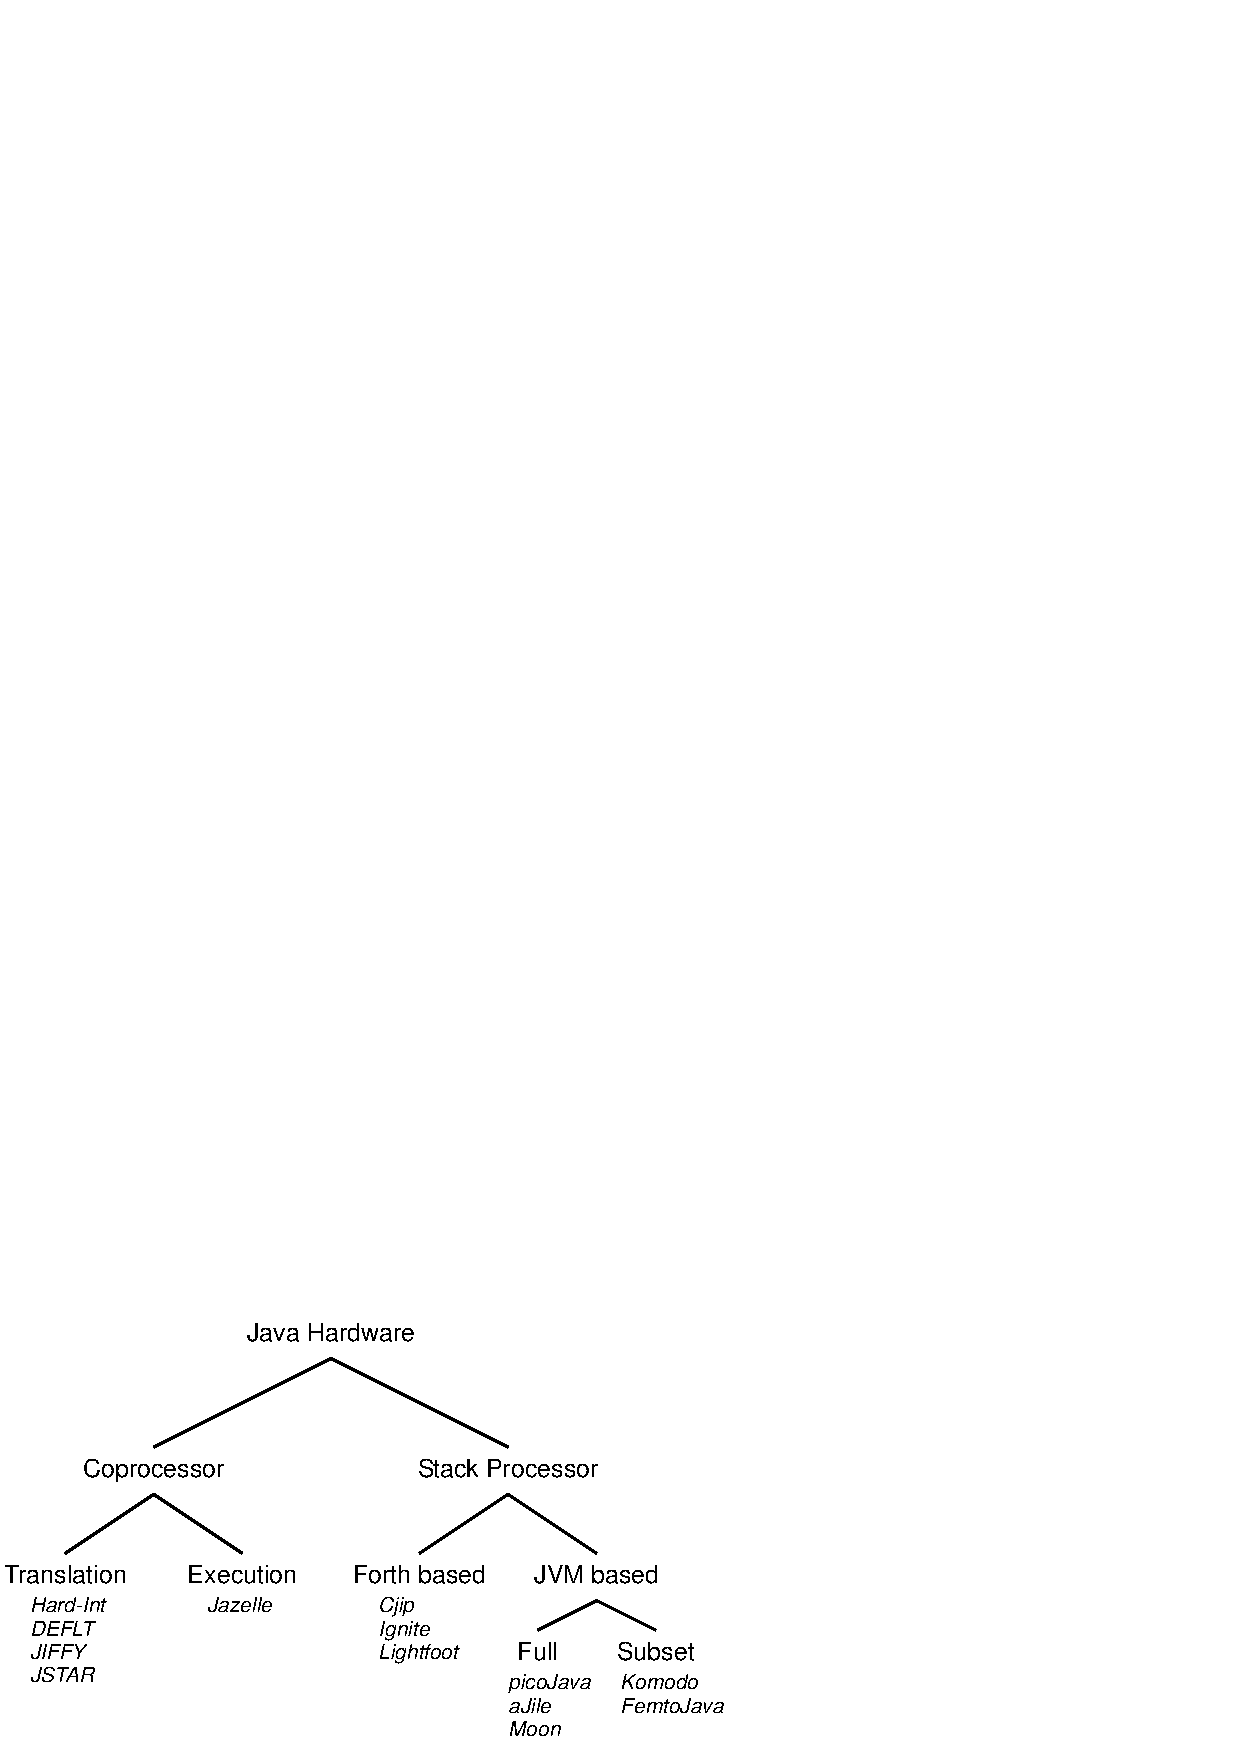
\includegraphics[scale=\picscale]{related/related_tree}
    \caption{Java hardware}
    \label{fig_related_tree}
\end{figure*}


There are problems in getting information about commercial products.
When new companies started developing Java processors, a lot of
information was available. This information was usually more of a
presentation of the concept, nevertheless it gave some insights into
how they approached the different design problems. However, at the
point at which the projects reached production quality, this
information quietly disappeared from their websites. It was replaced
with colorful marketing prospectuses about the wonderful world of
the new Java-enabled mobile phones. Only one company, aJile Ltd.,
presented information about their product in a refereed conference
paper.

Many research projects for a Java processor in an FPGA exists.
Examples can be found in \cite{Femto01}, \cite{Kim2000} and
\cite{368445}. These projects have much in common -- the basic
implementation of a stack machine with integer instructions is easy.
However, the realization of the complete JVM is the hard part and
therefore beyond the scope of these projects.

Other than the aJile processor and the Komodo project, no solution
addresses the problem of real-time predictability. For this reason,
as well as its availability, the aJile processor is used for
comparison with JOP.

\section{Summary}
\label{sec:related:summary}

In Table~\ref{tab:related:plus:minus}, features of selected Java
processors are compared. Category `Predictability' means how well
the processor is time-predictable. In category `Size', the chip size
is estimated and category `Performance' means average performance.
The category `JVM conformance' lists how complete the implementation
of the JVM specification \cite{jvm} is. The `Flexibility' parameter
indicates how well the processor can be adapted to different
application domains.

The assessment of the various parameters is, however, somewhat
subjective as the information is mainly derived from written
documentation. In Section~\ref{sec:performance}, the overall
performance of various Java systems, including the aJile processor,
is compared with JOP.

The last column of the table shows the features required for JOP.
This is, therefore, our research objective in a nutshell.

\begin{table}[htp]
    \centering
    \begin{tabular}{lccccc}
        \toprule
                        & picoJava & aJile   & Komodo  & FemtoJava & JOP     \\
        \midrule
        Predictability  & $--$     & $\cdot$ & $-$     & $\cdot$   & $++$    \\
        Size            & $--$     & $-$     & $+$     & $-$       & $++$    \\
        Performance     & $++$     & $+$     & $-$     & $--$      & $+$     \\
        JVM conformance & $++$     & $+$     & $-$     & $--$      & $\cdot$ \\
        Flexibility     & $--$     & $--$    & $+$     & $++$      & $++$    \\
        \bottomrule
    \end{tabular}
    \caption{Feature comparison of selected Java processors}
    \label{tab:related:plus:minus}
\end{table}

Due to the great variation in execution times for a trap, picoJava
is given a double minus in the `Predictability' category. picoJava
is also the largest processor in the list. However, its performance
and JVM compatibility are expected to be superior to those of other
processors.

The aJile processor is intended as a solution for real-time systems.
However, no information is available about bytecode execution times.
As this processor is a commercial product and has been on the market
for some time, it is expected that its JVM implementation would
conform to Java standards, as defined by Sun.

Komodos multithreading is similar to hyper-threading in modern
processors that are trying to hide latencies in instruction
fetching. However, this feature leads to very pessimistic WCET
values (in effect rendering the performance gain useless). The fact
that the pipeline clock is only a quarter of the system clock also
wastes a considerable amount of potential performance.

FemtoJava is given a double plus for flexibility, due to the
application-dependent generation of the processor. However,
FemtoJava is only a 16-bit processor and therefore not JVM
compliant. The resource usage is also very high, compared to the
minimal Java subset implemented and the low performance of the
processor.

So far, all processors in the list perform weakly in the area of
time-predictable execution of Java bytecodes. However, a low-level
analysis of execution times is of primary importance for WCET
analysis. Therefore, the main objective of JOP is to define and
implement a processor architecture that is as predictable as
possible. However, it is equally important that this does not result
in a low performance solution. Performance shall not suffer as a
result of the time-predictable architecture.

The second main aim of this work is to design a small processor.
Size and the resulting energy consumption are a main concern in
embedded systems. The proposed Java processor needs to be small
enough to be implemented in a low-cost FPGA device. With this
constraint, an implementation in an ASIC will also result in a very
small core that can be part of a larger system-on-a-chip.

The embedded market is diverse and one size does not fit all. A
configurable processor in which we can trade size for performance
provides the flexibility for a variety of application domains. The
aim of the architecture of JOP is to support this flexibility.

%\section{Derived Work}
%\label{sec:derived}
%
%Quite common for open-source projects are derived projects.
%Especially the research community appreciates open-source projects.
%Following list describes projects that are either completely based
%on JOP or influenced to a great extent.
%
%JOP triggered research on implementation of the JVM in hardware for
%real-time systems. The publications on JOP and also the fact that
%JOP is open-source made the project and ideas easy accessible for
%other researchers. Several research projects are directly or
%indirectly based on the research project JOP:
%
%\begin{itemize}
%    \item Lund -- Flavius
%    \item Dresden
%    \item Graz
%    \item Albertos MS thesis
%    \item \cite{conf/iscas/KoT07} JOP based dual-issue Javaprocessor
%    \item WCET work by Rasmus, Trevor, Elena, and upcoming CISS
%\end{itemize}
